\documentclass[conference]{IEEEtran}

% correct bad hyphenation here
\hyphenation{op-tical net-works semi-conduc-tor}
\usepackage{amsmath}
\usepackage{comment}
\usepackage{graphicx}
%\usepackage{cases}
%\usepackage{subeqnarray}

\usepackage{multicol}
\usepackage{lipsum}
\usepackage{mathtools}
\usepackage{cuted}

\usepackage{extpfeil}
\usepackage{mathpartir}
\usepackage[mathscr]{eucal}

\usepackage{hyperref}
\usepackage{cleveref}
\crefformat{section}{\S#2#1#3} % see manual of cleveref, section 8.2.1
\crefformat{subsection}{\S#2#1#3}
\crefformat{subsubsection}{\S#2#1#3}

\usepackage{algorithm}
\usepackage{algorithmicx}
\usepackage{algpseudocode}
\renewcommand{\algorithmicrequire}{\textbf{Input:}}
\renewcommand{\algorithmicensure}{\textbf{Output:}}

\usepackage{color}
\usepackage{xcolor}
\newcommand{\todo}[1]{\textcolor{red}{[TODO: #1]}}


\begin{document}
%
% paper title
% Titles are generally capitalized except for words such as a, an, and, as,
% at, but, by, for, in, nor, of, on, or, the, to and up, which are usually
% not capitalized unless they are the first or last word of the title.
% Linebreaks \\ can be used within to get better formatting as desired.
% Do not put math or special symbols in the title.
\title{Multiple Object Tracking with DeepSORT, LSTM, and More Kalman Filters}
%
%
% author names and IEEE memberships
% note positions of commas and nonbreaking spaces ( ~ ) LaTeX will not break
% a structure at a ~ so this keeps an author's name from being broken across
% two lines.
% use \thanks{} to gain access to the first footnote area
% a separate \thanks must be used for each paragraph as LaTeX2e's \thanks
% was not built to handle multiple paragraphs
%

\author{
    Shangning Xu,
    Zhongye Wang,
    Xinyu Zhan
}

% The paper headers
% \markboth{Journal of \LaTeX\ Class Files,~Vol.~13, No.~9, September~2014}%
% {Shell \MakeLowercase{\textit{et al.}}: Bare Demo of IEEEtran.cls for Journals}
% The only time the second header will appear is for the odd numbered pages
% after the title page when using the twoside option.
%
% *** Note that you probably will NOT want to include the author's ***
% *** name in the headers of peer review papers.                   ***
% You can use \ifCLASSOPTIONpeerreview for conditional compilation here if
% you desire.


% make the title area
\maketitle

% As a general rule, do not put math, special symbols or citations
% in the abstract or keywords.
\begin{abstract}
The abstract goes here.
\end{abstract}

% Note that keywords are not normally used for peerreview papers.
\begin{IEEEkeywords}
IEEEtran, journal, \LaTeX, paper, template.
\end{IEEEkeywords}


\IEEEpeerreviewmaketitle



\section{Introduction}

\IEEEPARstart{T}{his}

\section{Understanding and Re-implementing DeepSORT}

\section{Other Existing Advanced Techniques}
Despite of deep cosine features and multi-stage matching, there have been other more recent works on solving the multiple object tracking problem.
We mainly look into two innovative method that approaches the MOT problem using recurrent neural network and deep Hungarian network.

\subsection{Association LSTM}
The multi-object tracking in video can be considered as a task of process some sequence, which is natural to consider using recurrent neural networks to tackle the problem.
Lu \textit{et al.} \cite{lu2017online} implements an association LSTM which refines the detection and association feature from the time-invariant models.
We will briefly review their idea in this section.

In the traditional SORT algorithm, we will use Kalman filters to update the state of an object in the current frame.
Therefore, we can better match the future state of the object with the predicted one than matching the future state with the current state.
The association LSTM shares the similar idea, which not only refines the state of an object through prediction, but also predict the feature of each object.
More specifically, they let the LSTM to refine the feature extracted by some network, possibly the deep cosine features, by making the features of the same object across frames more similar while those of different objects more different.
The association loss \eqref{eq:assoc-loss} in their optimization goal reveals such objective.
\begin{equation}
    \mathcal{L}_{asso} = \sum_t \sum_{i,j} \theta_{ji}|\phi_{t-1}^i \cdot \phi_t^j|
    \label{eq:assoc-loss}
\end{equation}
where $\tilde{f}_t = \{\phi_t^1, \cdots, \phi_t^N\}$ is the refined feature for $N$ objects at time $t$, and $\theta_{ji} \in 0, 1$ is an indicator, which equals 1 iff. object $i$ at time $t-1$ should be associated with object $j$ at time $t$.
\todo{The associated objects is expected to have similar features, i.e., higher inner product values.
The higher loss means better performance.}

Figure~\ref{fig:lstm-struct} shows their model's structure.
Beside the association loss, there is another term in the loss function of the LSTM, the regression error.
They refines the states of objects through optimizing this term.

\begin{figure}[h]
    \centering
    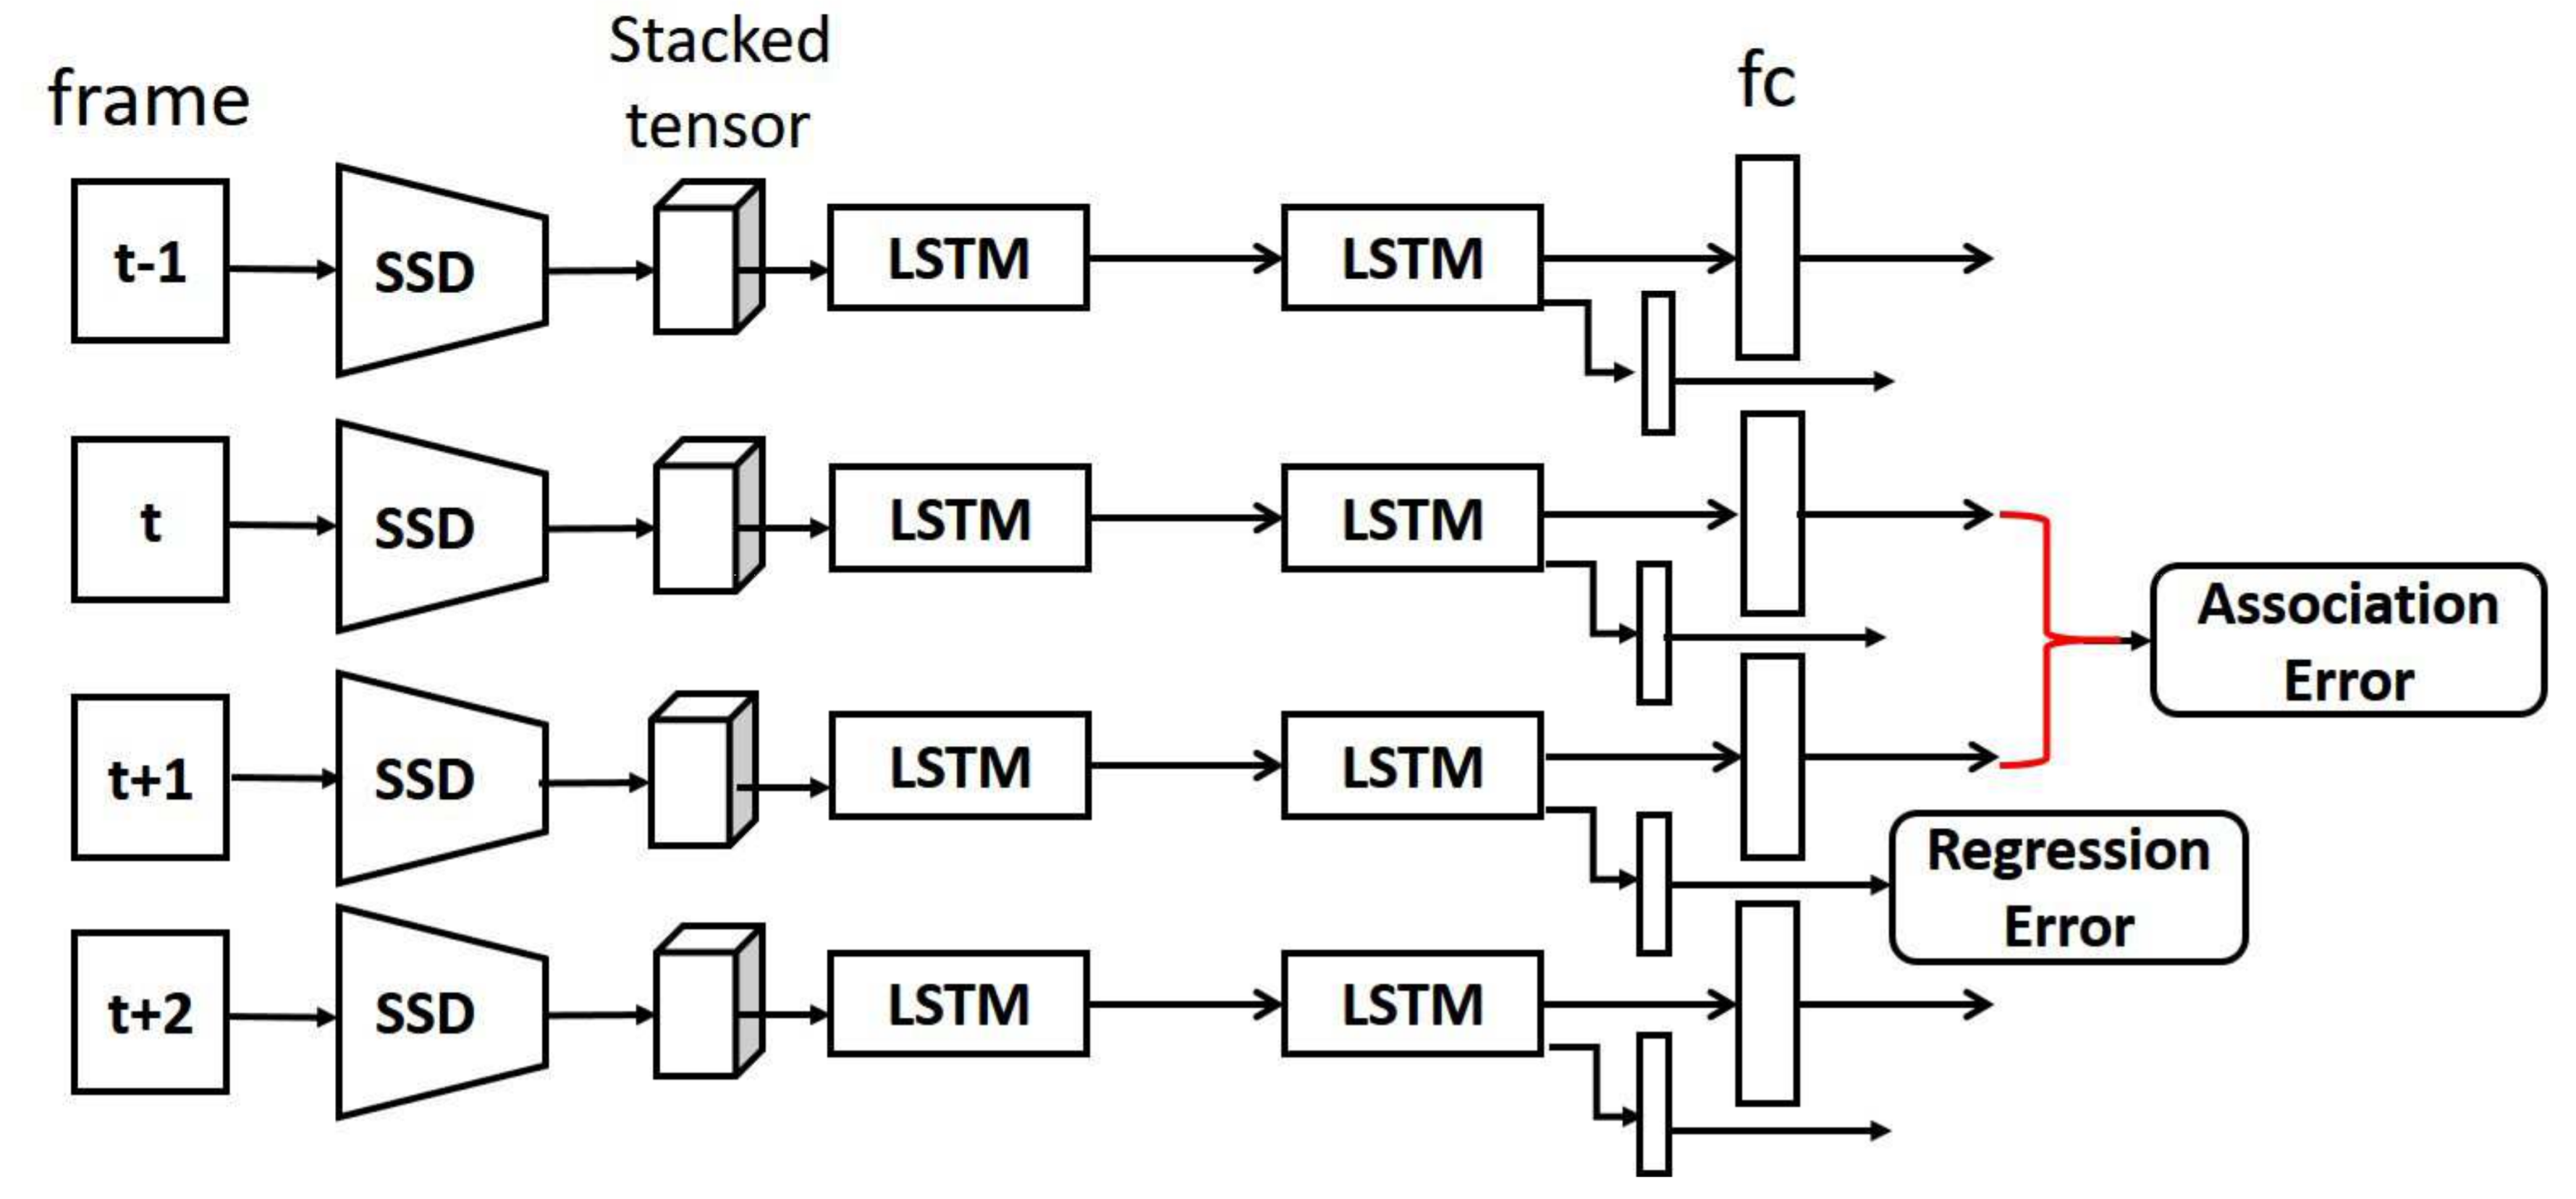
\includegraphics[width=0.99\linewidth]{fig/assoc_lstm.png}
    \caption{Association LSTM Structure\protect\footnotemark}
    \label{fig:lstm-struct}
\end{figure}
\footnotetext{From \cite{lu2017online}.}

As explained before, the functionality of the LSTM layer is similar to the Kalman filter.
However, the advantage of using LSTM is that it stores more information than the Kalman filter, which possesses only the knowledge of the previous frame due to the Markov assumption.
Every frame from the begin to the current one has their influences on the output of the LSTM at the current time stamp, allowing the network to fully utilize the information of the previous video.

We attempt to find some existing code implementing the idea but failed to do so.
We also try to implement the association LSTM ourselves but ended up with not enough computational resources to run experiments.
However, we are enlightened by the idea of carrying more information and predicting the transformation of features.
And we propose using Kalman filters to do the both in \cref{sec:our-work}.

\subsection{Deep Hungarian Network}
We have discussed how to upgrade the detection and feature extraction part so far, and now we move on to upgrade the matching algorithm.
The traditional approach is to formulate the problem as a bi-partite matching, where we need to matching objects in the previous frame with those in the current frame to minimizing the total distance (assuming the same object will not transform too much in both the spatial state and feature space), given the distance matrix.
The problem can be solved efficiently with Hungarian algorithm, the input and output of which are both matrices.
Xu \cite{xu2019deepmot} models the algorithm as a deep neural network, where more information and more complex computation can be performed to obtain the matching matrix.

\begin{figure*}
    \centering
    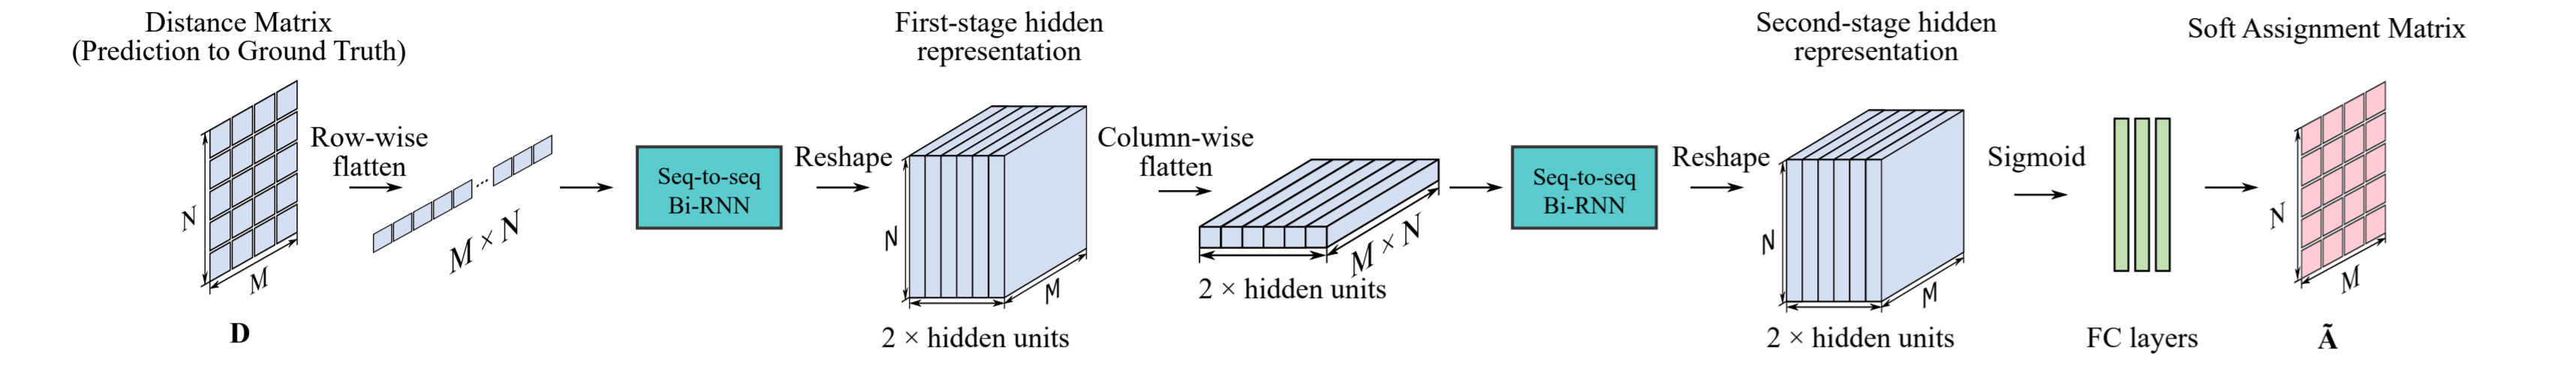
\includegraphics[width=\linewidth]{fig/dhn.png}
    \caption{The Structure of Deep Hungarian Network\protect\footnotemark}
    \label{fig:dhn-struct}
\end{figure*}

The structure of the deep Hungarian network they propose is shown in Figure~\ref{fig:dhn-struct}.
The input distance matrix is first flattened row-wise and processed by a bidirectional recurrent neural network to obtain a set of hidden feature representations.
After flatten the representations column-wise, they are then processed by another recurrent layer and some fully connected layers to obtain the soft assignment matrix.
The row-wise and column-wise flatten operations are to simulate the original Hungarian algorithm.

\footnotetext{From \cite{xu2019deepmot}.}

We had planned to integrate the refined feature matrix obtained from the association LSTM with the DHN, because the fixed output feature size is perfect for the input to the DHN.
But the failure to re-implement the former one causes us unable to try out such combination.
We run the code come along with the paper to get tracking performance on the training set of MOT16 and obtain Table~\ref{tab:eval-deepmot}.

\linespread{1.2}
\begin{table}[h]
    \caption{Evaluation Result of DeepMOT}
    \label{tab:eval-deepmot}
    \begin{tabular}{ccccccccc}
        \hline
        & MOTA & IDF1 & MT & ML & FP & FN & IDs\\\hline
        MOT16-02 & 21.5\% & 30.9\% & 6 & 25 & 1688 & 12240 & 77\\
        MOT16-04 & 15.7\% & 40.5\% & 11 & 28 & 16470 & 23435 & 166\\
        MOT16-05 & 15.8\% & 27.9\% & 3 & 88 & 677 & 5013 & 49\\
        MOT16-09 & 11.1\% & 41.4\% & 9 & 3 & 2788 & 1822 & 63\\
        MOT16-10 & 26.8\% & 40.5\% & 9 & 24 & 2243 & 6716 & 56\\
        MOT16-11 & 39.1\% & 47.4\% & 14 & 31 & 1826 & 3729 & 30\\
        MOT16-13 & 11.5\% & 30.6\% & 7 & 70 & 1279 & 8827 & 23\\
        OVERALL & 19.2\% & 38.4\% & 59 & 269 & 26971 & 61782 & 464\\\hline
    \end{tabular}
\end{table}
\linespread{1.0}

Compared to the deep SORT, the MOTA drops dramatically with lots of false positive and false negative increase.
The index switch count decreases, which could be caused due to the decrease of successful trackings, and therefore this index does not hold much meaning.

% The deep Hungarian network has many problems.
% It is a black box algorithm, whereas the Hungarian algorithm is a white box one and is proved to be reasonable.
% It is believed that 

\section{Our Work: Using More Kalman Filters}
\label{sec:our-work}
\subsection{Extended State Space}

Extending the state vector is a natural idea. A state space of higher dimensions should be able to characterize the state of object in video with more precision. The constant velocity model proposed by \cite{Wojke2017simple}, where the position, aspect ratio and height of a track changes linearly over time, is simple and should apply to most pedestrians, but fail to account for some complex cases, such as the one shown in Fig.~\ref{fig:example-of-nonlinearity}. Therefore, we augment the state space first with acceleration (2nd order) using the constant acceleration model and later higher order terms.

\begin{figure}[h]
    \centering
    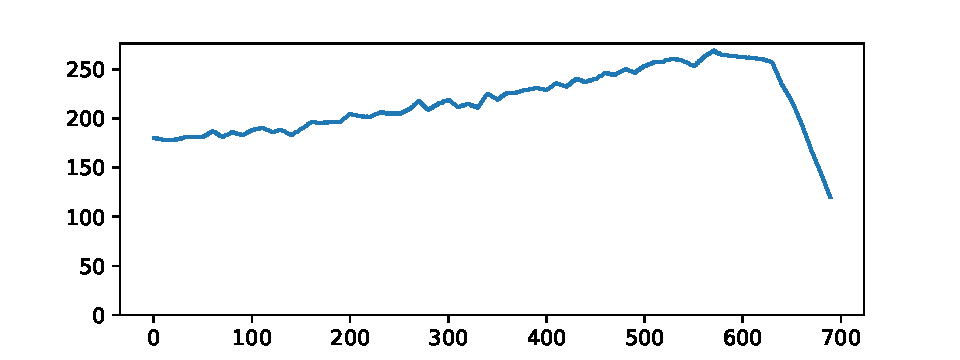
\includegraphics[width=\linewidth]{fig/accelerating-pedestrian-height-plot.pdf}
    \caption{An example of the nonlinear behavior of a state variable. The height of the pedestrian 70 in the sequence MOT16-02 is plotted against time. The pedestrian first moves towards camera and then exits the field of view.}
    \label{fig:example-of-nonlinearity}
\end{figure}

We give an example of augmenting the state space with acceleration below. The new state vector is
\[
    s = [x, y, a, h, v_x, v_y, v_a, v_h, a_x, a_y, a_a, a_h].
\]

Using the example of $x$-coordinate, the state-transition equation is
\[
    x_{k + 1} = x_k + v_{xk} \Delta t + \frac{1}{2} a_{xk} \Delta t^2.
\]

For the velocity, the equation is
\[
    v_{x, k + 1} = v_{xk} + a_{xk} \Delta t.
\]

The equations for other state variables are similar. The state-transition equation for the state vector is
\[
    s_{k + 1} = Fs_k + w_k,
\]
where $F$ is the new state-transition matrix
\[
    F = \begin{bmatrix}
        I_4 & \Delta t I_4 & \frac{1}{2} \Delta t^2 I_4\\
        \mathcal{O} & I_4 & \Delta t I_4\\
        \mathcal{O} & \mathcal{O} & I_4
    \end{bmatrix}
\]
and $w_k$ is noise.

The measurement matrix is
\[
    H = [I_4, \mathcal{O}, \mathcal{O}].
\]

In a similar fashion, the state vector with constant $k$-order terms is a $4k$-dimensional vector. The state-transition matrix is $4k \times 4k$ and the measurement matrix $4 \times 4k$ in this case.

\subsection{Filtering on Features}

\section{Conclusion}



\bibliographystyle{IEEEtran}
\bibliography{Ref}

\end{document}
